\documentclass[handout]{beamer}
\usetheme{Boadilla}
\usepackage{xcolor} \usepackage{caption}
\usepackage{tikz}
\usepackage{hyperref}

\title{Cellular Automata}
\subtitle{An introduction to Conway's Game of Life}
\author{Aniruddha Deb}
\institute{IIT Delhi}
\date{\today}

\captionsetup[figure]{font=footnotesize,labelfont=footnotesize}

\begin{document}

\begin{frame}
\titlepage
\end{frame}

\begin{frame}
\frametitle{Determinism and Non-Determinism}
\pause
\begin{flushleft}
A \textbf{Deterministic Algorithm} is an algorithm that repeatedly gives the
same set of outputs for a given set of outputs. An example is a simple function
$f(x) = x^2$
\end{flushleft}

\begin{center}
	\tikzset{every picture/.style={line width=0.75pt}} %set default line width to 0.75pt        
	
	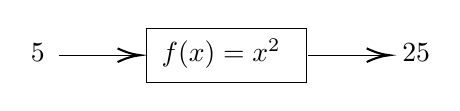
\begin{tikzpicture}[x=0.75pt,y=0.75pt,yscale=-1,xscale=1]
	
	%Shape: Rectangle [id:dp16197166944169683] 
	\draw   (221,80.97) -- (298,80.97) -- (298,106.97) -- (221,106.97) -- cycle ;
	%Straight Lines [id:da07695618334677845] 
	\draw    (179,93.97) -- (216,93.97) ;
	\draw [shift={(218,93.97)}, rotate = 180] [color={rgb, 255:red, 0; green, 0; blue, 0 }  ][line width=0.75]    (10.93,-3.29) .. controls (6.95,-1.4) and (3.31,-0.3) .. (0,0) .. controls (3.31,0.3) and (6.95,1.4) .. (10.93,3.29)   ;
	%Straight Lines [id:da47094111370416836] 
	\draw    (299,93.97) -- (336,93.97) ;
	\draw [shift={(338,93.97)}, rotate = 180] [color={rgb, 255:red, 0; green, 0; blue, 0 }  ][line width=0.75]    (10.93,-3.29) .. controls (6.95,-1.4) and (3.31,-0.3) .. (0,0) .. controls (3.31,0.3) and (6.95,1.4) .. (10.93,3.29)   ;
	
	% Text Node
	\draw (227,85) node [anchor=north west][inner sep=0.75pt]    {$f( x) =x^{2}$};
	% Text Node
	\draw (164,87) node [anchor=north west][inner sep=0.75pt]    {$5$};
	% Text Node
	\draw (343,87) node [anchor=north west][inner sep=0.75pt]    {$25$};
	\end{tikzpicture}
\end{center}

\pause
\begin{flushleft}
A \textbf{Nondeterministic Algorithm} is an algorithm that does not give 
repeatable outputs for a given input. An example is a cup in which n dice 
are rolled. ($g:\Bbb{N} \to \Bbb{N}^n$)
\end{flushleft}
\begin{center}
	\tikzset{every picture/.style={line width=0.75pt}} %set default line width to 0.75pt        
	
	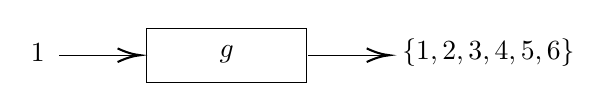
\begin{tikzpicture}[x=0.75pt,y=0.75pt,yscale=-1,xscale=1]
	
	%Shape: Rectangle [id:dp16197166944169683] 
	\draw   (221,80.97) -- (298,80.97) -- (298,106.97) -- (221,106.97) -- cycle ;
	%Straight Lines [id:da07695618334677845] 
	\draw    (179,93.97) -- (216,93.97) ;
	\draw [shift={(218,93.97)}, rotate = 180] [color={rgb, 255:red, 0; green, 0; blue, 0 }  ][line width=0.75]    (10.93,-3.29) .. controls (6.95,-1.4) and (3.31,-0.3) .. (0,0) .. controls (3.31,0.3) and (6.95,1.4) .. (10.93,3.29)   ;
	%Straight Lines [id:da47094111370416836] 
	\draw    (299,93.97) -- (336,93.97) ;
	\draw [shift={(338,93.97)}, rotate = 180] [color={rgb, 255:red, 0; green, 0; blue, 0 }  ][line width=0.75]    (10.93,-3.29) .. controls (6.95,-1.4) and (3.31,-0.3) .. (0,0) .. controls (3.31,0.3) and (6.95,1.4) .. (10.93,3.29)   ;
	
	% Text Node
	\draw (255,88) node [anchor=north west][inner sep=0.75pt]    {$g$};
	% Text Node
	\draw (164,87) node [anchor=north west][inner sep=0.75pt]    {$1$};
	% Text Node
	\draw (343,85) node [anchor=north west][inner sep=0.75pt]    {$\{1,2,3,4,5,6\}$};
	\end{tikzpicture}
\end{center}
\end{frame}

\begin{frame}
\frametitle{State Machines}
\pause
\begin{flushleft}
A \textbf{Finite State Machine} or \textbf{Finite State Automata} is a machine that can exist in exactly one of a finite
number of states at a given point in time, and can \textit{transition} between these states
as a result of inputs. A simple example is a switch.

\begin{center}
	\tikzset{every picture/.style={line width=0.75pt}} %set default line width to 0.75pt        
	
	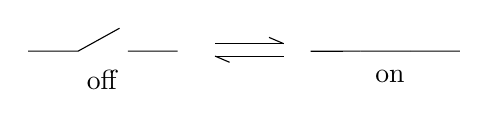
\begin{tikzpicture}[x=0.75pt,y=0.75pt,yscale=-1,xscale=1]
	%uncomment if require: \path (0,300); %set diagram left start at 0, and has height of 300
	
	%Straight Lines [id:da8818602134387576] 
	\draw    (14,20) -- (38,19.97) ;
	%Straight Lines [id:da6777788892413668] 
	\draw    (62,20) -- (86,19.97) ;
	%Straight Lines [id:da9797738416661963] 
	\draw    (38,20.03) -- (58,8.97) ;
	%Straight Lines [id:da978073320202391] 
	\draw    (150,20.05) -- (174,20.03) ;
	%Straight Lines [id:da7322212805692465] 
	\draw    (198,20) -- (222,19.97) ;
	%Straight Lines [id:da027703079406747655] 
	\draw    (174,20.03) -- (198,20) ;
	%Straight Lines [id:da7737672298064389] 
	\draw    (104,16.38) -- (137,16.38) ;
	%Straight Lines [id:da6321717459304543] 
	\draw    (104,22.38) -- (137,22.38) ;
	%Straight Lines [id:da0825108051498844] 
	\draw    (130,13.38) -- (137,16.38) ;
	%Straight Lines [id:da3024067774927739] 
	\draw    (104,22.38) -- (111,25.38) ;
	
	% Text Node
	\draw (41,27.97) node [anchor=north west][inner sep=0.75pt]   [align=left] {off};
	% Text Node
	\draw (180,27.97) node [anchor=north west][inner sep=0.75pt]   [align=left] {on};
	\end{tikzpicture}
\end{center}
\end{flushleft}
\pause
\begin{flushleft}
\textcolor{red}{Can we make an infinite state machine by combining infinite 
finite state machines?} \pause Theoretically yes, but practically no. We'll 
cover this in more detail when we go to Cellular Automata.
\end{flushleft}
\end{frame}

\begin{frame}
\frametitle{Deterministic and Nondeterministic Finite State Machines}
\pause
\begin{flushleft}
Combining both these concepts, a \textbf{Deterministic Finite State Automata (DFA)}
is one whose next state is uniquely determined by the current state. As an example,
a loading bar at n\% can only progress to a state at (n+1)\%
\end{flushleft}
\begin{center}
	\tikzset{every picture/.style={line width=0.75pt}} %set default line width to 0.75pt        
	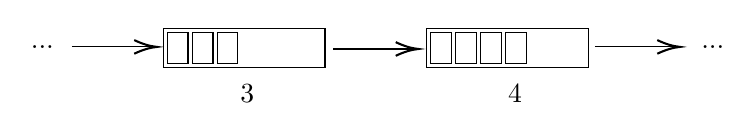
\begin{tikzpicture}[x=0.75pt,y=0.75pt,yscale=-1,xscale=1]
	%uncomment if require: \path (0,300); %set diagram left start at 0, and has height of 300
	
	%Shape: Rectangle [id:dp3055585661788678] 
	\draw   (79,65.96) -- (157,65.96) -- (157,84.96) -- (79,84.96) -- cycle ;
	%Shape: Rectangle [id:dp7931925075446689] 
	\draw   (81,68) -- (91,68) -- (91,82.96) -- (81,82.96) -- cycle ;
	%Shape: Rectangle [id:dp15280568454630794] 
	\draw   (93,68) -- (103,68) -- (103,82.96) -- (93,82.96) -- cycle ;
	%Shape: Rectangle [id:dp31013874960208776] 
	\draw   (105,68) -- (115,68) -- (115,82.96) -- (105,82.96) -- cycle ;
	%Straight Lines [id:da9983699961694059] 
	\draw    (161,75.96) -- (200,75.96) ;
	\draw [shift={(202,75.96)}, rotate = 180] [color={rgb, 255:red, 0; green, 0; blue, 0 }  ][line width=0.75]    (10.93,-3.29) .. controls (6.95,-1.4) and (3.31,-0.3) .. (0,0) .. controls (3.31,0.3) and (6.95,1.4) .. (10.93,3.29)   ;
	%Shape: Rectangle [id:dp30618464679355806] 
	\draw   (206,65.96) -- (284,65.96) -- (284,84.96) -- (206,84.96) -- cycle ;
	%Shape: Rectangle [id:dp1254421177009828] 
	\draw   (208,68) -- (218,68) -- (218,82.96) -- (208,82.96) -- cycle ;
	%Shape: Rectangle [id:dp6532262308883703] 
	\draw   (220,68) -- (230,68) -- (230,82.96) -- (220,82.96) -- cycle ;
	%Shape: Rectangle [id:dp6244802591256728] 
	\draw   (232,68) -- (242,68) -- (242,82.96) -- (232,82.96) -- cycle ;
	%Shape: Rectangle [id:dp8893622165126769] 
	\draw   (244,68) -- (254,68) -- (254,82.96) -- (244,82.96) -- cycle ;
	%Straight Lines [id:da025811777450731377] 
	\draw    (287,74.96) -- (326,74.96) ;
	\draw [shift={(328,74.96)}, rotate = 180] [color={rgb, 255:red, 0; green, 0; blue, 0 }  ][line width=0.75]    (10.93,-3.29) .. controls (6.95,-1.4) and (3.31,-0.3) .. (0,0) .. controls (3.31,0.3) and (6.95,1.4) .. (10.93,3.29)   ;
	%Straight Lines [id:da8840742882925454] 
	\draw    (35,74.96) -- (74,74.96) ;
	\draw [shift={(76,74.96)}, rotate = 180] [color={rgb, 255:red, 0; green, 0; blue, 0 }  ][line width=0.75]    (10.93,-3.29) .. controls (6.95,-1.4) and (3.31,-0.3) .. (0,0) .. controls (3.31,0.3) and (6.95,1.4) .. (10.93,3.29)   ;
	
	% Text Node
	\draw (14,73) node [anchor=north west][inner sep=0.75pt]   [align=left] {...};
	% Text Node
	\draw (337,73) node [anchor=north west][inner sep=0.75pt]   [align=left] {...};
	% Text Node
	\draw (115,91.76) node [anchor=north west][inner sep=0.75pt]   [align=left] {3};
	% Text Node
	\draw (244,91.96) node [anchor=north west][inner sep=0.75pt]   [align=left] {4};
	
	\end{tikzpicture}
\end{center}
\pause
\begin{flushleft}
In contrast, a \textbf{Nondeterministic Finite State Automata (NFA)} is one whose
next state is not uniquely determined by it's current state. An example would be 
the output of a dice roll: it's a NFA, because the number of states are finite,
and the next state is independent of the current state
\end{flushleft}
\begin{center}
	\tikzset{every picture/.style={line width=0.75pt}} %set default line width to 0.75pt        
	
	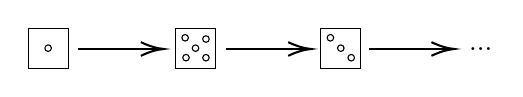
\begin{tikzpicture}[x=0.75pt,y=0.75pt,yscale=-1,xscale=1]
	%uncomment if require: \path (0,300); %set diagram left start at 0, and has height of 300
	
	%Shape: Square [id:dp9483231995146468] 
	\draw   (73.8,14.96) -- (93,14.96) -- (93,34.16) -- (73.8,34.16) -- cycle ;
	%Shape: Circle [id:dp7175213662466338] 
	\draw   (81.82,24.56) .. controls (81.82,23.69) and (82.53,22.98) .. (83.4,22.98) .. controls (84.27,22.98) and (84.98,23.69) .. (84.98,24.56) .. controls (84.98,25.44) and (84.27,26.14) .. (83.4,26.14) .. controls (82.53,26.14) and (81.82,25.44) .. (81.82,24.56) -- cycle ;
	%Shape: Square [id:dp054882816025298986] 
	\draw   (214.8,14.96) -- (234,14.96) -- (234,34.16) -- (214.8,34.16) -- cycle ;
	%Shape: Circle [id:dp9953687872245642] 
	\draw   (217.82,19.56) .. controls (217.82,18.69) and (218.53,17.98) .. (219.4,17.98) .. controls (220.27,17.98) and (220.98,18.69) .. (220.98,19.56) .. controls (220.98,20.44) and (220.27,21.14) .. (219.4,21.14) .. controls (218.53,21.14) and (217.82,20.44) .. (217.82,19.56) -- cycle ;
	%Shape: Circle [id:dp23952009990996714] 
	\draw   (222.82,24.56) .. controls (222.82,23.69) and (223.53,22.98) .. (224.4,22.98) .. controls (225.27,22.98) and (225.98,23.69) .. (225.98,24.56) .. controls (225.98,25.44) and (225.27,26.14) .. (224.4,26.14) .. controls (223.53,26.14) and (222.82,25.44) .. (222.82,24.56) -- cycle ;
	%Shape: Circle [id:dp43257373267717214] 
	\draw   (227.84,29.16) .. controls (227.84,28.29) and (228.55,27.58) .. (229.42,27.58) .. controls (230.29,27.58) and (231,28.29) .. (231,29.16) .. controls (231,30.04) and (230.29,30.74) .. (229.42,30.74) .. controls (228.55,30.74) and (227.84,30.04) .. (227.84,29.16) -- cycle ;
	%Shape: Square [id:dp6920394020811227] 
	\draw   (144.8,14.96) -- (164,14.96) -- (164,34.16) -- (144.8,34.16) -- cycle ;
	%Shape: Circle [id:dp27320036187554386] 
	\draw   (147.82,19.56) .. controls (147.82,18.69) and (148.53,17.98) .. (149.4,17.98) .. controls (150.27,17.98) and (150.98,18.69) .. (150.98,19.56) .. controls (150.98,20.44) and (150.27,21.14) .. (149.4,21.14) .. controls (148.53,21.14) and (147.82,20.44) .. (147.82,19.56) -- cycle ;
	%Shape: Circle [id:dp19167432458357347] 
	\draw   (152.82,24.56) .. controls (152.82,23.69) and (153.53,22.98) .. (154.4,22.98) .. controls (155.27,22.98) and (155.98,23.69) .. (155.98,24.56) .. controls (155.98,25.44) and (155.27,26.14) .. (154.4,26.14) .. controls (153.53,26.14) and (152.82,25.44) .. (152.82,24.56) -- cycle ;
	%Shape: Circle [id:dp853176913471684] 
	\draw   (157.84,29.16) .. controls (157.84,28.29) and (158.55,27.58) .. (159.42,27.58) .. controls (160.29,27.58) and (161,28.29) .. (161,29.16) .. controls (161,30.04) and (160.29,30.74) .. (159.42,30.74) .. controls (158.55,30.74) and (157.84,30.04) .. (157.84,29.16) -- cycle ;
	%Shape: Circle [id:dp570530892686927] 
	\draw   (157.84,20.16) .. controls (157.84,19.29) and (158.55,18.58) .. (159.42,18.58) .. controls (160.29,18.58) and (161,19.29) .. (161,20.16) .. controls (161,21.04) and (160.29,21.74) .. (159.42,21.74) .. controls (158.55,21.74) and (157.84,21.04) .. (157.84,20.16) -- cycle ;
	%Shape: Circle [id:dp3387031524896331] 
	\draw   (148.24,29.14) .. controls (148.24,28.27) and (148.95,27.56) .. (149.82,27.56) .. controls (150.69,27.56) and (151.4,28.27) .. (151.4,29.14) .. controls (151.4,30.02) and (150.69,30.72) .. (149.82,30.72) .. controls (148.95,30.72) and (148.24,30.02) .. (148.24,29.14) -- cycle ;
	%Straight Lines [id:da4600687500874969] 
	\draw    (98,24.96) -- (137,24.96) ;
	\draw [shift={(139,24.96)}, rotate = 180] [color={rgb, 255:red, 0; green, 0; blue, 0 }  ][line width=0.75]    (10.93,-3.29) .. controls (6.95,-1.4) and (3.31,-0.3) .. (0,0) .. controls (3.31,0.3) and (6.95,1.4) .. (10.93,3.29)   ;
	%Straight Lines [id:da9667807125932639] 
	\draw    (169,24.96) -- (208,24.96) ;
	\draw [shift={(210,24.96)}, rotate = 180] [color={rgb, 255:red, 0; green, 0; blue, 0 }  ][line width=0.75]    (10.93,-3.29) .. controls (6.95,-1.4) and (3.31,-0.3) .. (0,0) .. controls (3.31,0.3) and (6.95,1.4) .. (10.93,3.29)   ;
	%Straight Lines [id:da6611074785868187] 
	\draw    (238,24.96) -- (277,24.96) ;
	\draw [shift={(279,24.96)}, rotate = 180] [color={rgb, 255:red, 0; green, 0; blue, 0 }  ][line width=0.75]    (10.93,-3.29) .. controls (6.95,-1.4) and (3.31,-0.3) .. (0,0) .. controls (3.31,0.3) and (6.95,1.4) .. (10.93,3.29)   ;
	
	% Text Node
	\draw (285,23) node [anchor=north west][inner sep=0.75pt]   [align=left] {...};
	\end{tikzpicture}
\end{center}
\end{frame}

\begin{frame}
\frametitle{Cellular Automata}
\begin{flushleft}
A \textbf{Cellular Automata} is a collection of cells (FSM with on/off state),
each of which changes it's state based on the states of it's neighbouring cells. \\~\\
\pause
Elementary cellular automata simply involve a 1D grid (a continuous array 
of cells). I'll not be covering those now. Instead, let's focus on 2D grids. \\~\\
\pause
Each cell has two types of neighbourhoods: \textbf{Moore} and \textbf{Von Neumann}. 
Rules (either Deterministic or Nondeterministic) based on these neighbourhoods 
determine the next state of the cell.
\end{flushleft}

\begin{center}
\begin{figure}
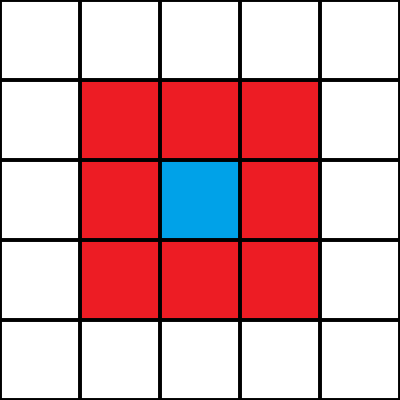
\includegraphics[scale=0.15]{img/moore_nbd}
\hspace{5em}
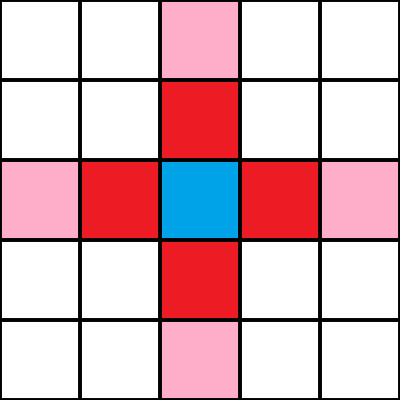
\includegraphics[scale=0.15]{img/vn_nbd}
\caption{Moore(L) and Von Neumann(R) neighbourhoods}
\end{figure}
\end{center}

\end{frame}

\begin{frame}
\frametitle{Bounds for Cellular Automata}
\begin{flushleft}

We'll cover Life in a while, but a question: 
\end{flushleft}
\pause
\begin{center}\begin{Large}\textcolor{red}{
Are Cellular Automata Finite state or Infinite state?}
\end{Large}\end{center}
\pause

\begin{flushleft}
Theoretically, nothing prevents cellular automata from being infinite-state
automata. However, they would have a countably infinite number of states,
which makes things (theoretically) simpler. For all practical purposes,
however, cellular automata are finite and are bounded by the memory space of
the computer simulating them. \\~\\
\pause
If we do have to bound an automata, we generally impose a different set of 
conditions on the boundary: something like reflection or stasis or vanishing
conditions.
\end{flushleft}
\end{frame}

\begin{frame}
\frametitle{Conway's Game of Life   {\tiny (finally!)}}
\begin{flushleft}
\textbf{Conway's Game of Life} is a Cellular Automata that follows the following
rules on the Moore neighbourhood $N$ of a cell $C$:
\pause
\begin{itemize}
\item{If $C$ is dead, and exactly 3 cells in $N$ are alive, then $C$ becomes
alive in the next iteration i.e. $C$ \textbf{is born}}
\pause
\item{If $C$ is alive, and exactly 2 or 3 cells in $N$ are alive, then $C$ remains 
alive in the next iteration i.e. $C$ \textbf{survives}}
\end{itemize}
\pause
These rules can be summarized as \textbf{B3/S23}. Variations of this rule set
give several other automata. What's interesting about Life is that it's stable:
it doesn't explode or decay very fast. \\~\\
\pause
Few other things: Life is Turing complete   {\tiny (proof left as an exercise)},
and Life is Undecidable: you cannot predict the initial state from the final
state, or directly compute n states into the future (as a consequence of the 
Halting problem).
\end{flushleft}
\end{frame}

\begin{frame}
\frametitle{Interesting patterns in Life}
\begin{itemize}
\pause
\item{Still Life}
\pause
\item{Oscillators}
\pause
\item{Gliders}
\pause
\item{Spaceships}
\pause
\item{Methuselahs}
\pause
\item{Glider Gun}
\end{itemize}
\end{frame}

\begin{frame}
\frametitle{Further reading/watching}
\begin{itemize}
\item{Numberphile video on Life (With Conway himself): \url{https://www.youtube.com/watch?v=R9Plq-D1gEk}}
\item{LifeWiki, the reference on all Game of Life Patterns: \url{https://www.conwaylife.com/wiki/}}
\item{Golly, an open-source program for simulating life: \url{http://golly.sourceforge.net}}
\item{PyGameOfLife, a Game of Life program implemented in Python: \url{https://github.com/Aniruddha-Deb/PyGameOfLife}}
\end{itemize}
\end{frame}

\end{document}
